\section{Introduction}

\begin{frame}{Breadth-First Search}
    \begin{itemize}
        \item Breadth-First Search is a fundamental algorithm in graph analysis
        \item Used in many algorithms: Dijkstra, Maximum Flow, MSP...
        \item Vertices are labeled based on the \alert{distance} from a given \textit{source} vertex
    \end{itemize}
    \begin{figure}
        \centering
        \begin{subfigure}[b]{0.32\textwidth}
            \centering
            \includegraphics[width=0.8\linewidth]{images/Collaboration network.png}
            \caption{Social network}
        \end{subfigure}
        \begin{subfigure}[b]{0.32\textwidth}
            \centering
            \includegraphics[width=1.05\linewidth]{images/roadnet.png}
            \caption{Road network}
        \end{subfigure}
    \end{figure}
\end{frame}

\begin{frame}{Breadth-First Search Example}
\centering
\begin{tikzpicture}[
    every node/.style={circle, draw},
    node distance=1.5cm,
  ]

  % Nodes
  \node[fill=white] (A) {A};
  \node[right=of A, fill=white] (B) {B};
  \node[below=of B, fill=white] (C) {C};
  \node[right=of B, fill=white] (D) {D};

  % Edges
  \draw (A) -- (B);
  \draw (A) -- (C);
  \draw (B) -- (C);
  \draw (B) -- (D);

  % Animations
  \uncover<2->{
    \node[fill=myred] (A) {A};
    \node[draw=myred, left=0.2cm of A, rectangle, align=center, font=\footnotesize] (boxA) {Distance = 0\\Parent = NULL};
  }

  \uncover<3->{
    \node[fill=myblue] (B) [right=of A] {B};
    \node[fill=myyellow] (C) [below=of B] {C};
    \node[draw=myblue, above=0.2cm of B, rectangle, align=center, font=\footnotesize] (boxB) {Distance = 1\\Parent = A};
    \node[draw=myyellow, below=0.2cm of C, rectangle, align=center, font=\footnotesize] (boxC) {Distance = 1\\Parent = A};
  }

  \uncover<4->{
    \node[fill=mygreen] (D) [right=of B] {D};
    \node[draw=mygreen, below=0.2cm of D, rectangle, align=center, font=\footnotesize] (boxD) {Distance = 2\\Parent = B};
  }
\end{tikzpicture}
\begin{minipage}{\textwidth}
    \centering
    \vspace{0.5cm}
    \only<1>{\textbf{Source vertex:} A}
    \only<2>{\textbf{Frontier:} A}
    \only<3>{\textbf{Frontier:} B, C}
    \only<4>{\textbf{Frontier:} D}
\end{minipage} 
\end{frame}

\begin{frame}{Modern Computer Architectures}
\begin{itemize}
    \item BFS has \bigO{V + E} time and space complexity (under RAM model)
    \item<2-> In practice, it is a \textbf{memory-bound algorithm} % no actual computation happening
    \begin{itemize}
        \item Algorithm exhibits poor cache locality
    \end{itemize}
    \item<3-> CPUs exhibit growing amount of \textbf{parallelism}...
    \item<4-> ...and new architectures are coming to the market (ARM, RISC-V)
\end{itemize}
\uncover<3->{
\begin{figure}
    \centering
    \vspace{-3mm}
    \includegraphics[width=0.6\linewidth]{images/cores.png}
    \vspace{-4mm}
    \caption{\scriptsize Evolution of core counts per socket for AMD and Intel processors}
    \label{fig:cores}
\end{figure}
}
\end{frame}

\begin{frame}{Contents}
\begin{itemize}
    \item New \textit{MergedCSR} data structure
    \item Two optimized parallel implementations (OpenMP and pthreads)
    \pause
    \item Evaluated against GAP Benchmark suite
    \item Speedups compared on three different architectures (AMD x86, RISC-V, ARM)
\end{itemize}
\begin{figure}
    \centering
    \begin{subfigure}[c]{0.4\textwidth}
    \centering
        \includegraphics[height=2.5cm]{images/gapbs.png}
        \caption{GAP suite logo}
    \end{subfigure}
    \begin{subfigure}[c]{0.4\textwidth}
        \centering
        \includegraphics[height=2.5cm]{images/architectures.png}
        \caption{Compared architectures}
    \end{subfigure}
\end{figure}
\end{frame}